%pæn (projekttitel på forside!!!)
%vi skal også beskrive interne regler (fx bødekasse)
%sekvensdiagram
%designmockups


\documentclass[11pt,a4paper]{report}

\setlength{\textwidth}{165mm}
\setlength{\textheight}{240mm}
\setlength{\parindent}{0mm} % S{\aa} meget rykkes ind efter afsnit
\setlength{\parskip}{\baselineskip}
\setlength{\headheight}{0mm}
\setlength{\headsep}{0mm}
\setlength{\hoffset}{-2.5mm}
\setlength{\voffset}{0mm}
\setlength{\footskip}{15mm}
\setlength{\oddsidemargin}{0mm}
\setlength{\topmargin}{0mm}
\setlength{\evensidemargin}{0mm}



\usepackage{courier} % The font we use.
\usepackage[a4paper, hmargin={2.8cm, 2.8cm}, vmargin={2.5cm, 2.5cm}]{geometry}
\usepackage{eso-pic} % \AddToShipoutPicture
\usepackage{graphicx} % \includegraphics
\usepackage[english]{babel}
\usepackage[utf8]{inputenc}
\usepackage{appendix}
\usepackage{amsfonts,amsmath,amssymb}
\usepackage[colorinlistoftodos]{todonotes}
%\usepackage{gauss} % Gauss Matrix
\usepackage{float} % This will allow precise picture placement, use [H].
\usepackage{enumitem}

\usepackage{microtype}
\usepackage[super]{nth}
\usepackage{booktabs} % This package provide some additional commands to enhance the quality of tables in LaTeX.
\usepackage{listings} % code parsing.
\PassOptionsToPackage{hyphens}{url}\usepackage{hyperref}
\lstset{language=bash} % Set bash syntax.
\newcommand{\code}[1]{\texttt{#1}}

\newlist{SubItemList}{itemize}{1}
\setlist[SubItemList]{label={$-$}}

\let\OldItem\item
\newcommand{\SubItemStart}[1]{%
    \let\item\SubItemEnd
    \begin{SubItemList}[resume]%
        \OldItem #1%
}
\newcommand{\SubItemMiddle}[1]{%
    \OldItem #1%
}
\newcommand{\SubItemEnd}[1]{%
    \end{SubItemList}%
    \let\item\OldItem
    \item #1%
}
\newcommand*{\SubItem}[1]{%
    \let\SubItem\SubItemMiddle%
    \SubItemStart{#1}%
}%

\newcommand{\BAR}{%
  \hspace{-\arraycolsep}%
  \strut\vrule % the `\vrule` is as high and deep as a strut
  \hspace{-\arraycolsep}%
}

\author{\Large{Sven Frenzel (\href{mailto:sven@frenzel.dk}{sven@frenzel.dk}) - 130793 - cdn769}\\
\Large{Mads Gram (\href{mailto:mgmadsgram@gmail.com}{mgmadsgram@gmail.com})  - 081293 - wtc324}\\
\Large{Thorkil Værge (\href{mailto:thorkilk@gmail.com}{thorkilk@gmail.com}) - 150287 - wng750} \\ \\
\Large{Instructor: Kasper Passov }}

\title{
\vspace{3cm}
\Large{Second Partial Assignment - ProjDat}
}

\begin{document}

%% Change `ku-farve` to `nat-farve` to use SCIENCE's old colors or
%% `natbio-farve` to use SCIENCE's new colors and logo.
\AddToShipoutPicture*{\put(0,0){\includegraphics*[viewport=0 0 700 600]{include/natbio-farve}}}
\AddToShipoutPicture*{\put(0,602){\includegraphics*[viewport=0 600 700 1600]{include/natbio-farve}}}

%% Change `ku-en` to `nat-en` to use the `Faculty of Science` header
\AddToShipoutPicture*{\put(0,0){\includegraphics*{include/nat-en}}}

\clearpage\maketitle
\thispagestyle{empty}

\newpage
\tableofcontents{}
\thispagestyle{empty}


\newpage

\chapter{Literature Review}\label{ch:Literature_Review}

\section{Gould \& Lewis -- Designing for Usability: key principles and what
designers think}
\subsection{Résumé}
This article from 1985 can be divided into two different parts: Actual recommendations for systems design and a survey to estimate how often this process is followed. The principles for good software design are outlined as follows:
\begin{itemize}
\item Early focus on users: designers must understand who the users will be, and this understanding is preferably obtained through actual interaction between the developer and end user.
\item Empirical measurements: Also known as user testing. Early in the process intended users should use simulations and prototypes to carry out real work and their performance should influence the system through $\rightarrow$
\item Iterative design: Problems during for example testing and user testing should influence design decisions which logically, in the design process, are done ``before'' testing. Iterative design breaks down the strict connection betwen time and logic.
\end{itemize}
The survey finds that most programmers do not mention these three points and when they do, they often misunderstand or misrepresent the actual meaning of the points. They may think that they are following the recommendations but they are not. Several reasons that the recommendations are not followed is listed and among these are that the programmers sometimes do not take responsibility for the entire project but only for the modules that are assigned to them. The article also emphasises the limitations of reason and stresses the need for empirical data in design decisions. This is illustrated by some good but counterintuitive interface design decisions from the design of a voice mail system from IBM called ``ADS''.

Behavioral goals should be developed for the end user and these goals should be testable. A goal could for example be that 80 \% of the users should be able to solve some task within a given amount of time without help or other instructions than what is given through the interaction with the system. In the design process, modularization of the program is also recommended.
\subsection{Analysis and Perspective}
This article differs from other litterature that we have read in that it focuses on the limitations of reason and the need for empirical observations when making design decisions. It stresses that the optimal design choice can in some situations not be deducted but must be found through interaction with end users. On page 306 the article makes a very bold prediction that ease of use will become important when selling computer devices. The fulfillment of that prophecy has, among others, been achived by Apple with their iPod and iPhone.

Due to this article's strong focus on how to make good decisions for the user interface, it reads as much like a guide in human–computer interaction (HCI) as a guide in systems design.
\subsection{Perspectivation to Work on dikukeys}
This article focuses a lot on interaction with the end user. Actual user testing has not been done during the work on dikukeys and it is probably not possible to do before a minimally working website is done. It is something that was not even on our list of planned tasks but that is something we should definitely include in the system. A user test can still influence the design process even though it is performed late since we follow an iterative process (AGILE).

The reading of this article likely means that we will test a prototype on users sooner than we would otherwise have.
\newpage
\section{Parnas \& Clements -- A Rational Design Process: How and Why to
Fake it}
\subsection{Résumé}
The article explains that a perfectly rational design process would be preferable so that a computer program or service could be derived rationally in the same sense that theorems are derived from axioms in mathematics. But for several reasons, this process cannot be followed perfectly: customers do not know their exact requirements before some of the functionality is presented, during the programming new discoveries are made which invalidate previous beliefs so we must backtrack, the complexity is too overwhelming to include all elements before programming and testing is initiated, and unpredictable external changes may occur.

Nonetheless, there are still many reasons for attempting to follow a rational design process. Some of the reasons which are mentioned in the article are: simply attempting, makes us come closer to the rational design process and reduces backtracking; standardization of the design process makes it easier for employees to join an ongoing project.

The rational design process which should be followed is defined by the work products:
\begin{itemize}
\item A requirements document: a place to record the desired behavior of the program.
\item A module structure: A division of the program and work programming into logical subentities. For large systems, it is preferably made as a tree structure.
\item Module interfaces: Formalized description of how the modules interact, an interface specification. Like an API for each module.
\item Uses hierarchy: A binary matrix which lists all the dependencies of the individual modules. Especially useful during post-release maintenance.
\item Internal module structure: Documentation of design decisions for each module that has been defined in module structure.
\item The actual program: The source code of the program for delivery. Should not contain redundant comments which have already been described in the documentation mentioned above.
\end{itemize}
If any changes during the design phase, programming phase, or post-delivery phase invalidate a design document, then all the documentation should be ``faked'' to look as if the change had been the original design. This design documentation is similar to a mathematical proof where the logical design and not the temporal development is the guiding force. Repetitions should be avoided in the documentation by asking: ``what questions should this specific document answer'', before it is written.
\subsection{Analysis and Perspective}
If this design process is followed then the documentation will follow the logical structure outlined above. Decisions made whilst coding or testing can feed into changes in the requirements document so the design process becomes iterative. This document thus encompasses many important elements of the Agile Manifesto\cite{beck} written 15 years later. For some of the group members of dikukeys, a temporal process in the documentation instead of a logical guiding force seems more intuitive but this article makes a very convincing case why the logical structure is preferable both during the programming phase and especially during the maintenance phase.
\subsection{Perspectivation to Work on dikukeys}
Due to the very rigid and comprehensive structure of these partial assignments, not all recommendations in this article can be followed: Many of the sections we are asked to write forces us to repeat ourselves which should be avoided according to this article. The repetition for instance occurred in the ``FACTOR analysis'' of partial assignment number 1. To follow the recommendation in this article, the repetitions should be avoided in the final report.

When this has been said, a positive effect of the many, sometimes redundant, questions we are asked to answer, is that we become familiar with many different concepts and work methods which we would not have been taught if we had followed the recipe outlined in this article. After reading this article, we were motivated to follow this design process rigorously but it is not certain that the requirements set forth by the teachers will allow us to do that in the final report.

We believe that this article has made a more compelling argument for the AGILE design process than any argument that we have read previously.
\chapter{Project Report}\label{ch:Project_Report}

\section{Abstract}\label{sec:Abstract}
The system developed [system], as part of this project, is a module of a system developed by Oleksander Shturmov [Online TA]. The purpose of the system is to validate the identity of a student submitting an assignment to Online TA. \\
This is done by mapping OpenPGP keys provided by the students with their KU Username. This mapping is achieved through a website on which a student registers themselves. This website is part of the system developed. Furthermore an API is provided to Online TA for integration. The system is developed for the Department of Computer Science at the University of Copenhagen [DIKU] represented by Oleksander Shturmov. Oleksander Shturmov has shown a desire to replace the currently used Learning Management System [LMS] \textit{its Learning} with a platform that can facilitate automatically evaluation of programming assignments. For this he needed a system to make sure that a given assignment was handed in by the student claiming to have handed it in. This is the system we are developing.
A prototype of the system is available at \url{http://dikukeys.dk:8081/app}.\footnote{Currently a valid email address has to be entered, even though the website suggest, that only a KU Username is needed. Please do not enter an email address that is hosted on an Office 365 solution, as you will not receive the email. We are working on not getting caught by their spam filter.}

\section{Purpose and Framework for the Project}\label{sec:Purpose_Framework}
This definition is based on the FACTOR criteria which serves the purpose of providing the structure for a systems definition.
\begin{itemize}
\item \textbf{F}unctionality: The purpose of the system is to allow specific students and employees at the University of Copenhagen to map their username to a public PGP key and store these records in a database maintained by the customer. The system must also allow the same users to replace their public key in case they lose the corresponding private key. The mappings should be readable by specific users with privileged access through some login mechanism.
\item \textbf{A}pplication domain: The system will be used by students to upload their OpenPGP key and by teaching assistants to match hand-ins that have been signed by a student's OpenPGP key with a KU Username. It is used when TAs receive hand-ins by the students and before the grading commences.
\item \textbf{C}onditions: Most students are not likely to have experience with OpenPGP so it should be as simple as possible to upload a key and the system must be forgiving, meaning that if a student loses his private PGP key, they must be able to upload a new public key. Instructions to guide the students through the various tasks of creating and uploading a key must be available. The system must allow other software to access the mappings.
\item \textbf{T}echnology: Servers with a UNIX-like OS will run the system, and modern browsers will be used for the front-end. The system will be written in golang to the widest extent possible but will also utilize SQL, HTML, CSS. It will also use existing software in the form of nginx for the webserver.
\item \textbf{O}bjects: The primary objects in the problem domain are students, TAs, and their uniquely identifying keys, in this case OpenPGP-keys.
\item \textbf{R}esponsibility: The system's main responsiblity is to maintain a table with a mapping from KU Usernames to corresponding OpenPGP public keys. It must also allow other privileged software to read from this table.
\end{itemize}

\renewcommand{\thesubsection}{\thesection.\alph{subsection}}
\section{Specification of Requirements for the IT Solution}\label{sec:Requirements}
\subsection{Functional and Non-functional Requirements}
\subsubsection{Functional Requirements}\label{subsubsec:Functional_Req}
The functional requirements describe features which are essential to the success of the project and describe actual functionality for the end-user or system administrator.
\begin{itemize}
\item The system must map a KU Username to an OpenPGP public key.
\item Users must be able to upload their own public key to the service.
\item If a user loses their private key, a method for replacing the public key must exist.
\item The initial registration of a key, and the replacement of a key, is authenticated through the KU email system.
\item The data has to be accessible to privileged software through a defined API.
\item The KU usernames registered in this system must not be accessible for non-privileged users and software.
\item A guide for creating key pairs needs to be available on the website, possibly as shell script. This guide should also explain how to derive an SSH key from an OpenPGP key.
\item A way for an administrator to send email invitations for joining the system to a list of students.
\end{itemize}

\subsubsection{Non-functional Requirements}\label{subsubsec:Non_Functional_Req}
Non-functional requirements are system requirements which do not describe the actual functionality but instead describe either non-essential systems, internal architecture, or design.
\begin{itemize}
\item The back-end should be written in golang.
\item The front-end should be Javascript and/or HTML5, which ever is safest and most easy to use.
\item The system should be browser independent.
\item The system must be compliant with all standards and regulations imposed by the Government of Denmark and the University of Copenhagen. These regulations concern privacy and restriction of access to the KU usernames that are part of the system. Specifically, the KU usernames in the system must not be accessible to non-privileged users\footnote{The priveliged users are system administrators, university professors, and TAs.}.
\item The customer has decreed that the software be licensed under a MIT-like license which will be provided by the customer.
\item The system should be able to decode the different .csv-formats (comma, semicolon, tab) for student lists.
\item The front-end must be responsive in its layout. This is achieved by using Bootstrap\footnote{Bootstrap can be found on \href{http://getbootstrap.com/}{http://getbootstrap.com/}}.
\end{itemize}

\subsection{Use Case Overview Model}\label{subsec:Use_case_model}

Figure \ref{fig:use_case_diagram_high_level} represents a high-level model which shows which actions are available for the different users: students and teachers.

% Think about moving text and diagram under the specific use case, rather than here!
In Figure \ref{fig:use_case_diagram_example} the use case for uploading a key is defined by listing which actions the student must perform to have his key stored on the dikukeys server.

\begin{figure}[H]
\centering
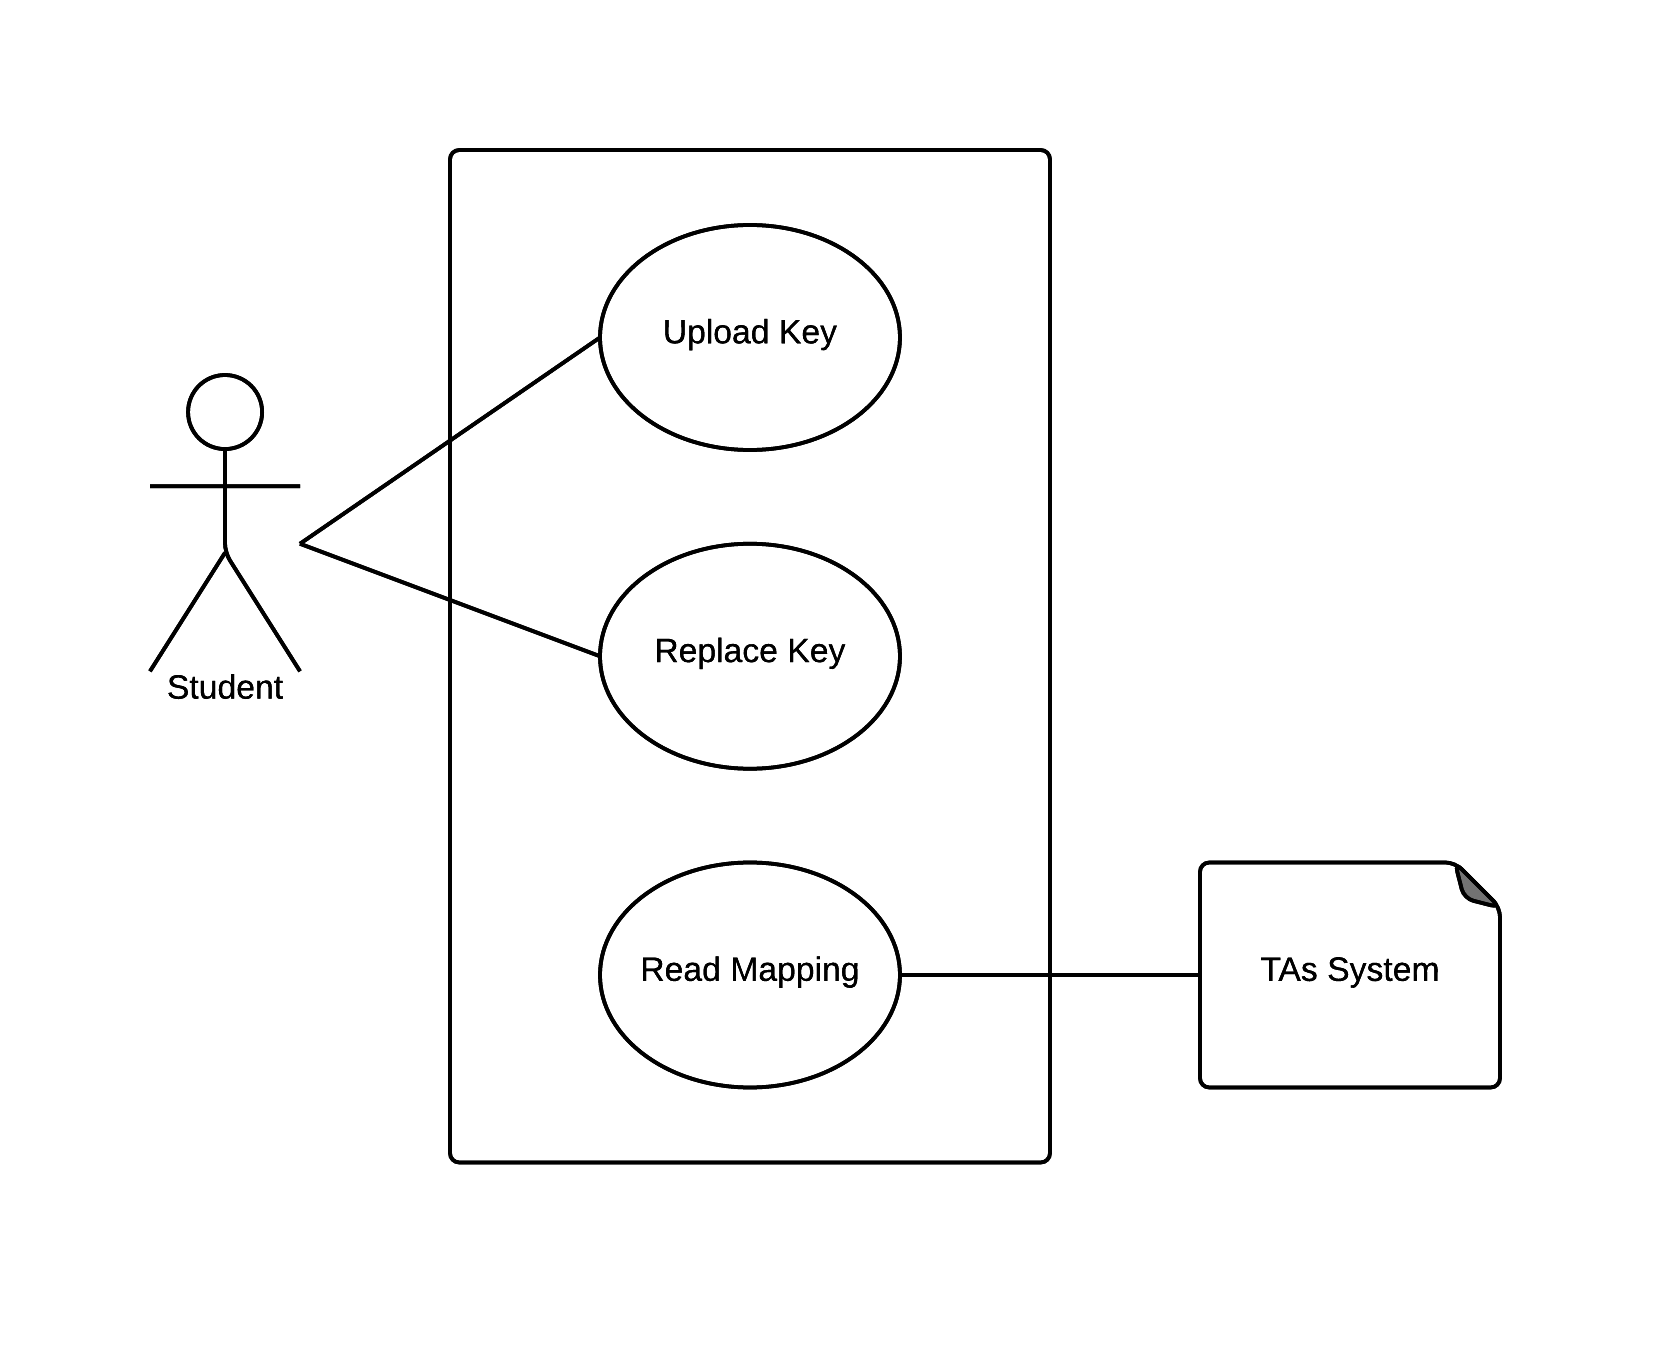
\includegraphics[width=0.7\textwidth]{pictures/use_case_pksu_del2_b_high}
\caption{High-level use case diagram. Students can upload or replace a public key, and teachers (TAs, professors, and system administrators) can pull data from the lists.}
\label{fig:use_case_diagram_high_level}
\end{figure}


\subsection{Specific Use Case Models}\label{subsec:Specific_Use_case_model}
Here, three different use cases for the system is showed by listing the actions of the relevant actors. The use cases for uploading a key, replacing a key, and sending out an invitation for joining the system are listed.
\subsubsection{Use Case: Upload Key}
\begin{tabular}{l p{0.8\textwidth}}
    \toprule
    \textit{Use case name} & Upload Key \\
    \midrule
    \textit{Participating} & Students \\
    \textit{actors} & \\
    \midrule
    \textit{Flow of events} &
    \vspace{-6.7mm} \begin{enumerate}
        \item Student follows link to dikukeys in invitation email OR student goes to dikukeys directly.
        \item Student enters their KU Username into a form.
        \item Server sends activation email to student's KU-email address.
        \item Student follows link in key activation email.
        \item Student posts their public key into a form or generates a key pair in the browser.
        \item Server sends email which confirms that a key has been uploaded.
    \end{enumerate}
    \\
    \midrule
    \textit{Entry condition} & User has an active KU ID. \\
                             & User is not registered in the system. \\
    \midrule
    \textit{Exit conditions} & User is registered in the system with a public key. \\
    \bottomrule
\end{tabular}
-
\begin{figure}[H]
    \centering
    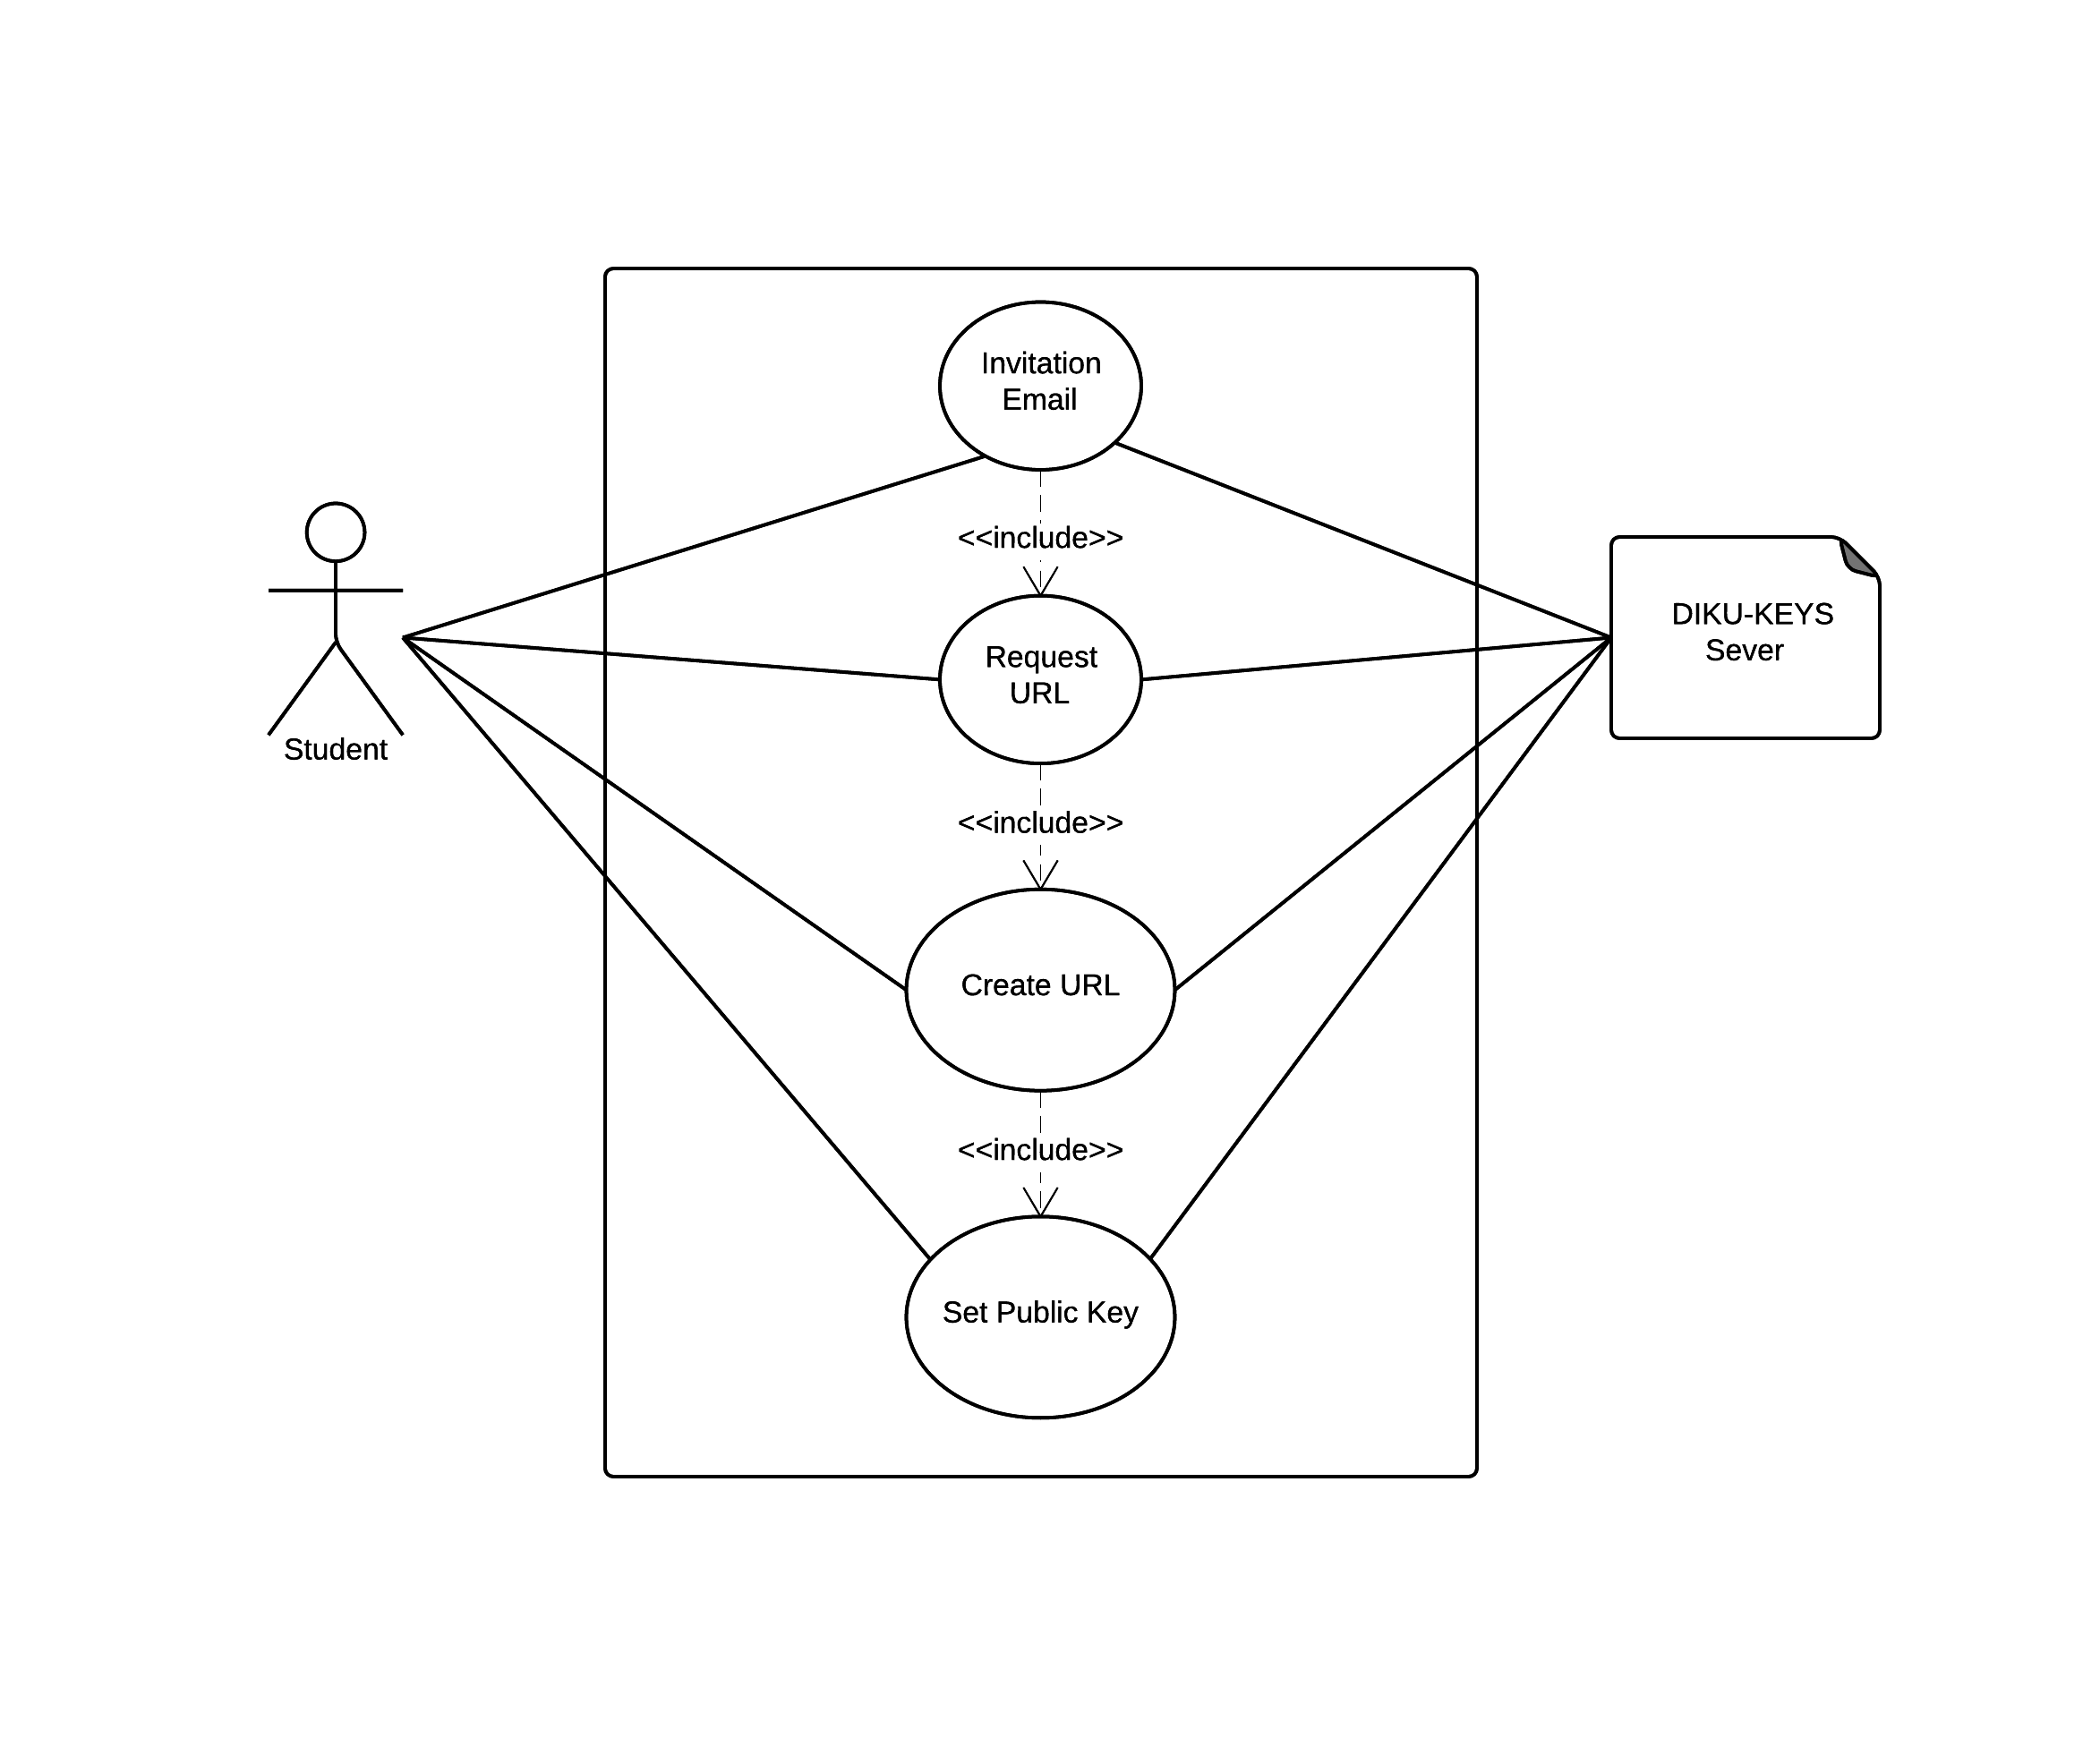
\includegraphics[width=0.7\textwidth]{pictures/use_case_pksu_del2_b_example}
    \caption{Flow diagram for uploading a key.}
    \label{fig:use_case_diagram_example}
\end{figure}

\subsubsection{Use Case: Replace Key}
\begin{tabular}{l p{0.8\textwidth}}
    \toprule
    \textit{Use case name} & Replace Key \\
    \midrule
    \textit{Participating} & Students \\
    \textit{actors} & \\
    \midrule
    \textit{Flow of events} &
    \vspace{-6.7mm} \begin{enumerate}
        \item Student goes to dikukeys.
        \item Student enters their KU Username into a form.
        \item Server sends key replacement email to student's KU email address.
        \item Student follows link in key replacement email.
        \item Student posts their new public key into a form or generates a new key pair in the browser.
        \item Server sends email which confirms that the new key has been uploaded.
    \end{enumerate}
    \\
    \midrule
    \textit{Entry condition} & Student is already a registered user in the system but with an invalid public key. \\
    \midrule
    \textit{Exit conditions} & A new public key has been registered to the student. \\
    \bottomrule
\end{tabular}

\subsubsection{Use Case: Invite Group of Students}
\begin{tabular}{l p{0.8\textwidth}}
    \toprule
    \textit{Use case name} & Invite Group of Students\\
    \midrule
    \textit{Participating} & Course director \\
    \textit{actors} & System administrator \\
    \midrule
    \textit{Flow of events} &
    \vspace{-6.7mm} \begin{enumerate}
        \item Course director sends a list of students and information about course to system administrator.
        \item System administator submits list of students course-information to the server via ssh.
        \item Server checks if students already are in the system. Depending on the answer one of the following two happens:
        \item
        \begin{enumerate}
            \item If the student is \textbf{not} already registered, the server sends an invitation email to the KU email address of the student.
            \item If the student is already registered, the server sends an email to the student informing them that the system will be used in this course.
        \end{enumerate}
    \end{enumerate}
    \\
    \midrule
    \textit{Entry condition} & User is course director \\
                             & User has a list of students \\
    \midrule
    \textit{Exit conditions} & All students from the list have either received an invitation to the system or have been informed that the system will be used in this course. \\
    \bottomrule
\end{tabular}

\subsection{Class Diagram of Solution Domain}\label{subsec:class_diagram}
A class diagram, where five different classes have been identified, has been made. The classes which are contained constitute different parts of software as well as the server on which the system is hosted. The classes have been identified according to the BCE model. The BCE analysis is especially relevant for the sequence diagram since it shows which classes can interact with the user. Only the boundary (B) classes can do that. And only interactions with the entity classes can change the state of the system through a user input.
\begin{figure}[H]
    \centering
    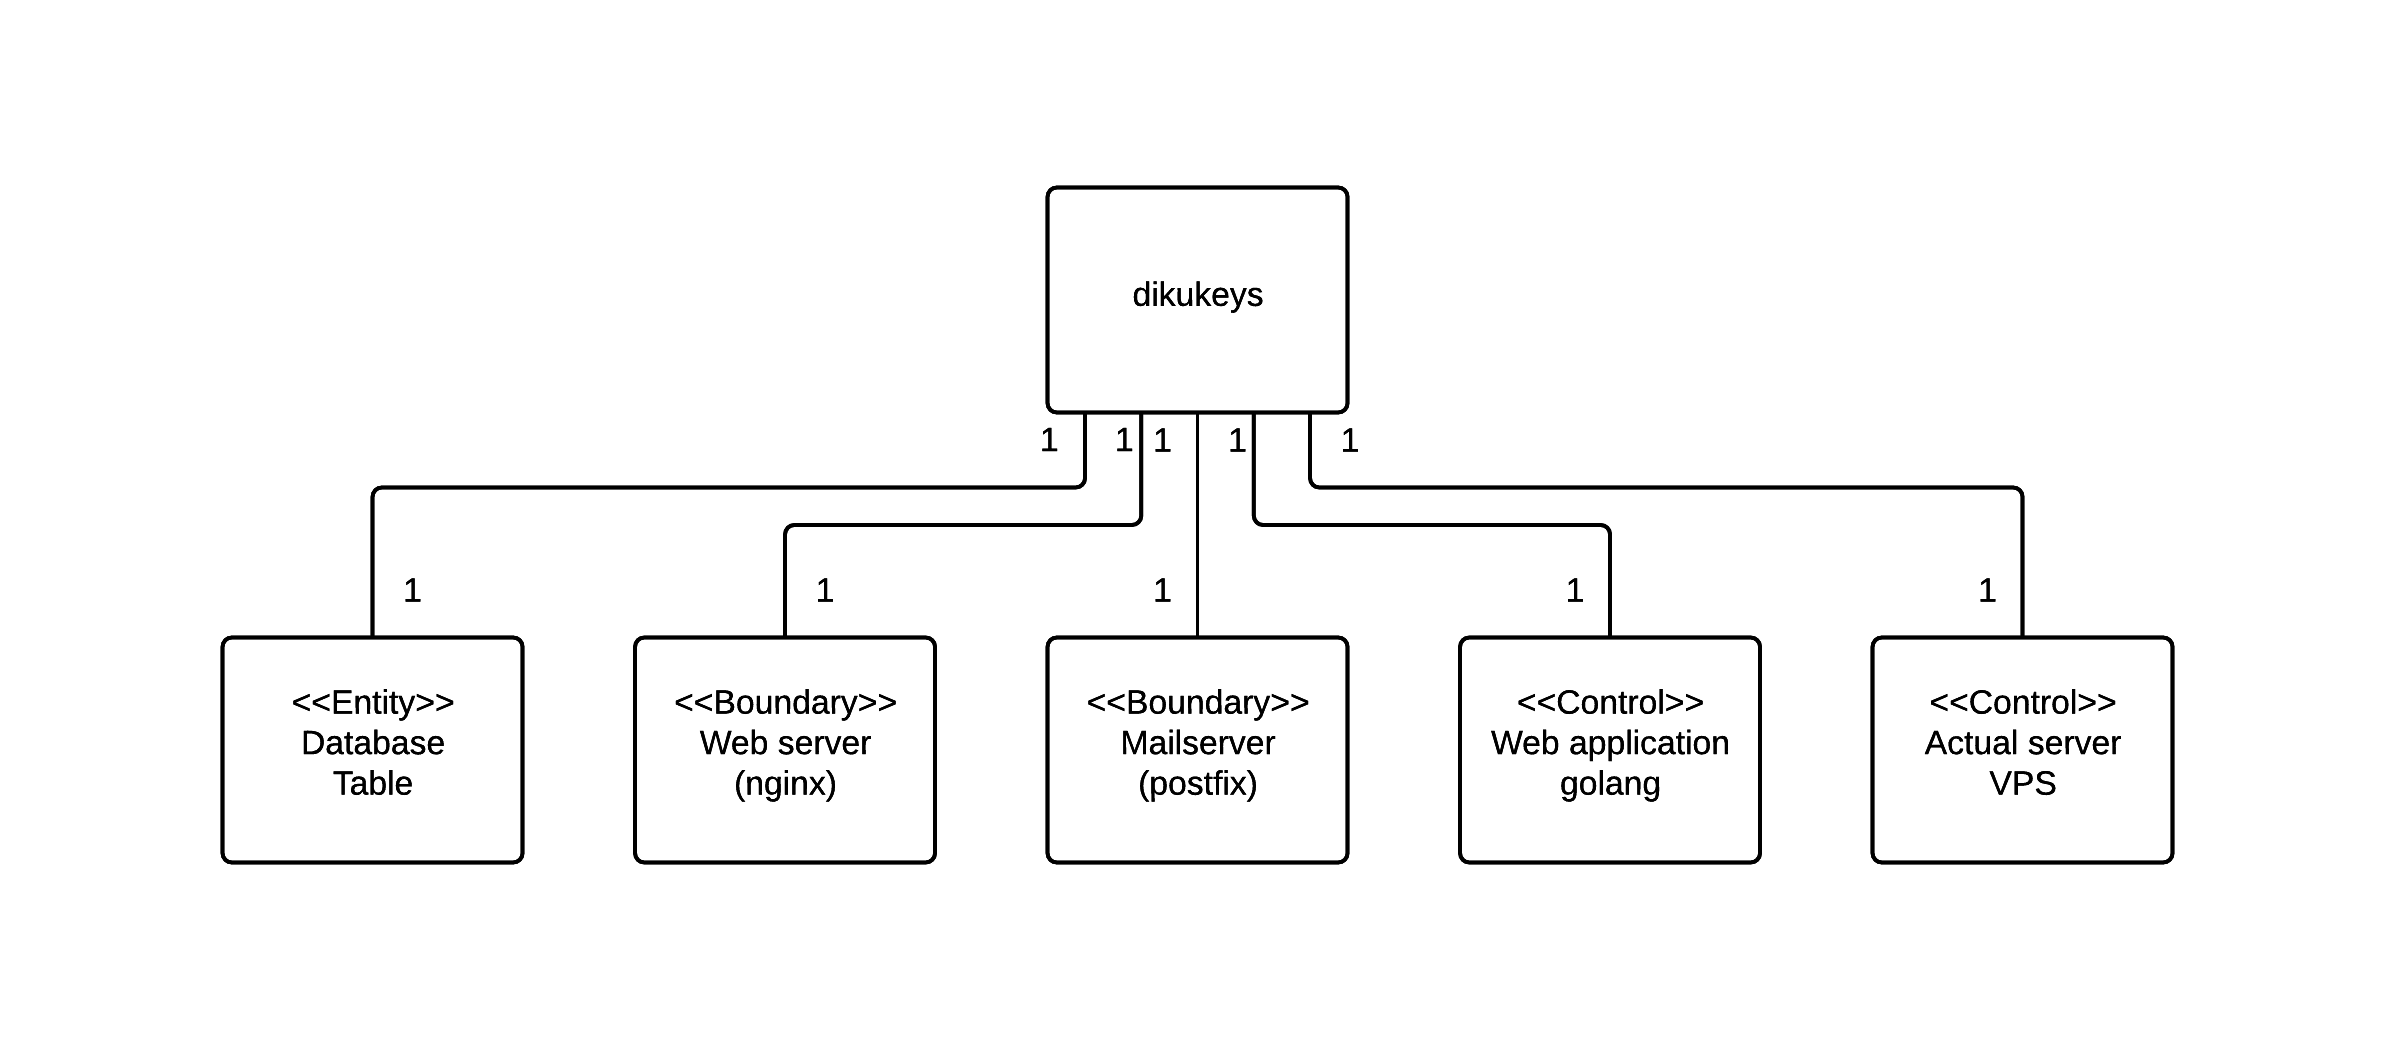
\includegraphics[width=\textwidth]{pictures/class_diagram}
    \caption{Class diagram of solution domain. The dikuserver solution consists of the classes which normally consitute a web solution: the HTTP handler (web server), the logic which creates the HTML code, the database which can permanently record user input, and an email server which is an alternative way of communicating with the user and whose purpose it is to validate the identity of the user.}     -    \label{fig:class_diagram}
\end{figure}
\subsection*{}

\subsection{Sequence Diagrams of Use Case}\label{subsec:Sequence_diagram_Use_case_model}
Figure \ref{fig:sequence_diagram} shows the logical flow between the logical classes identified in the class diagram above. Only the boundary classes can interact directly with the user.
\begin{figure}[H]
    \centering
    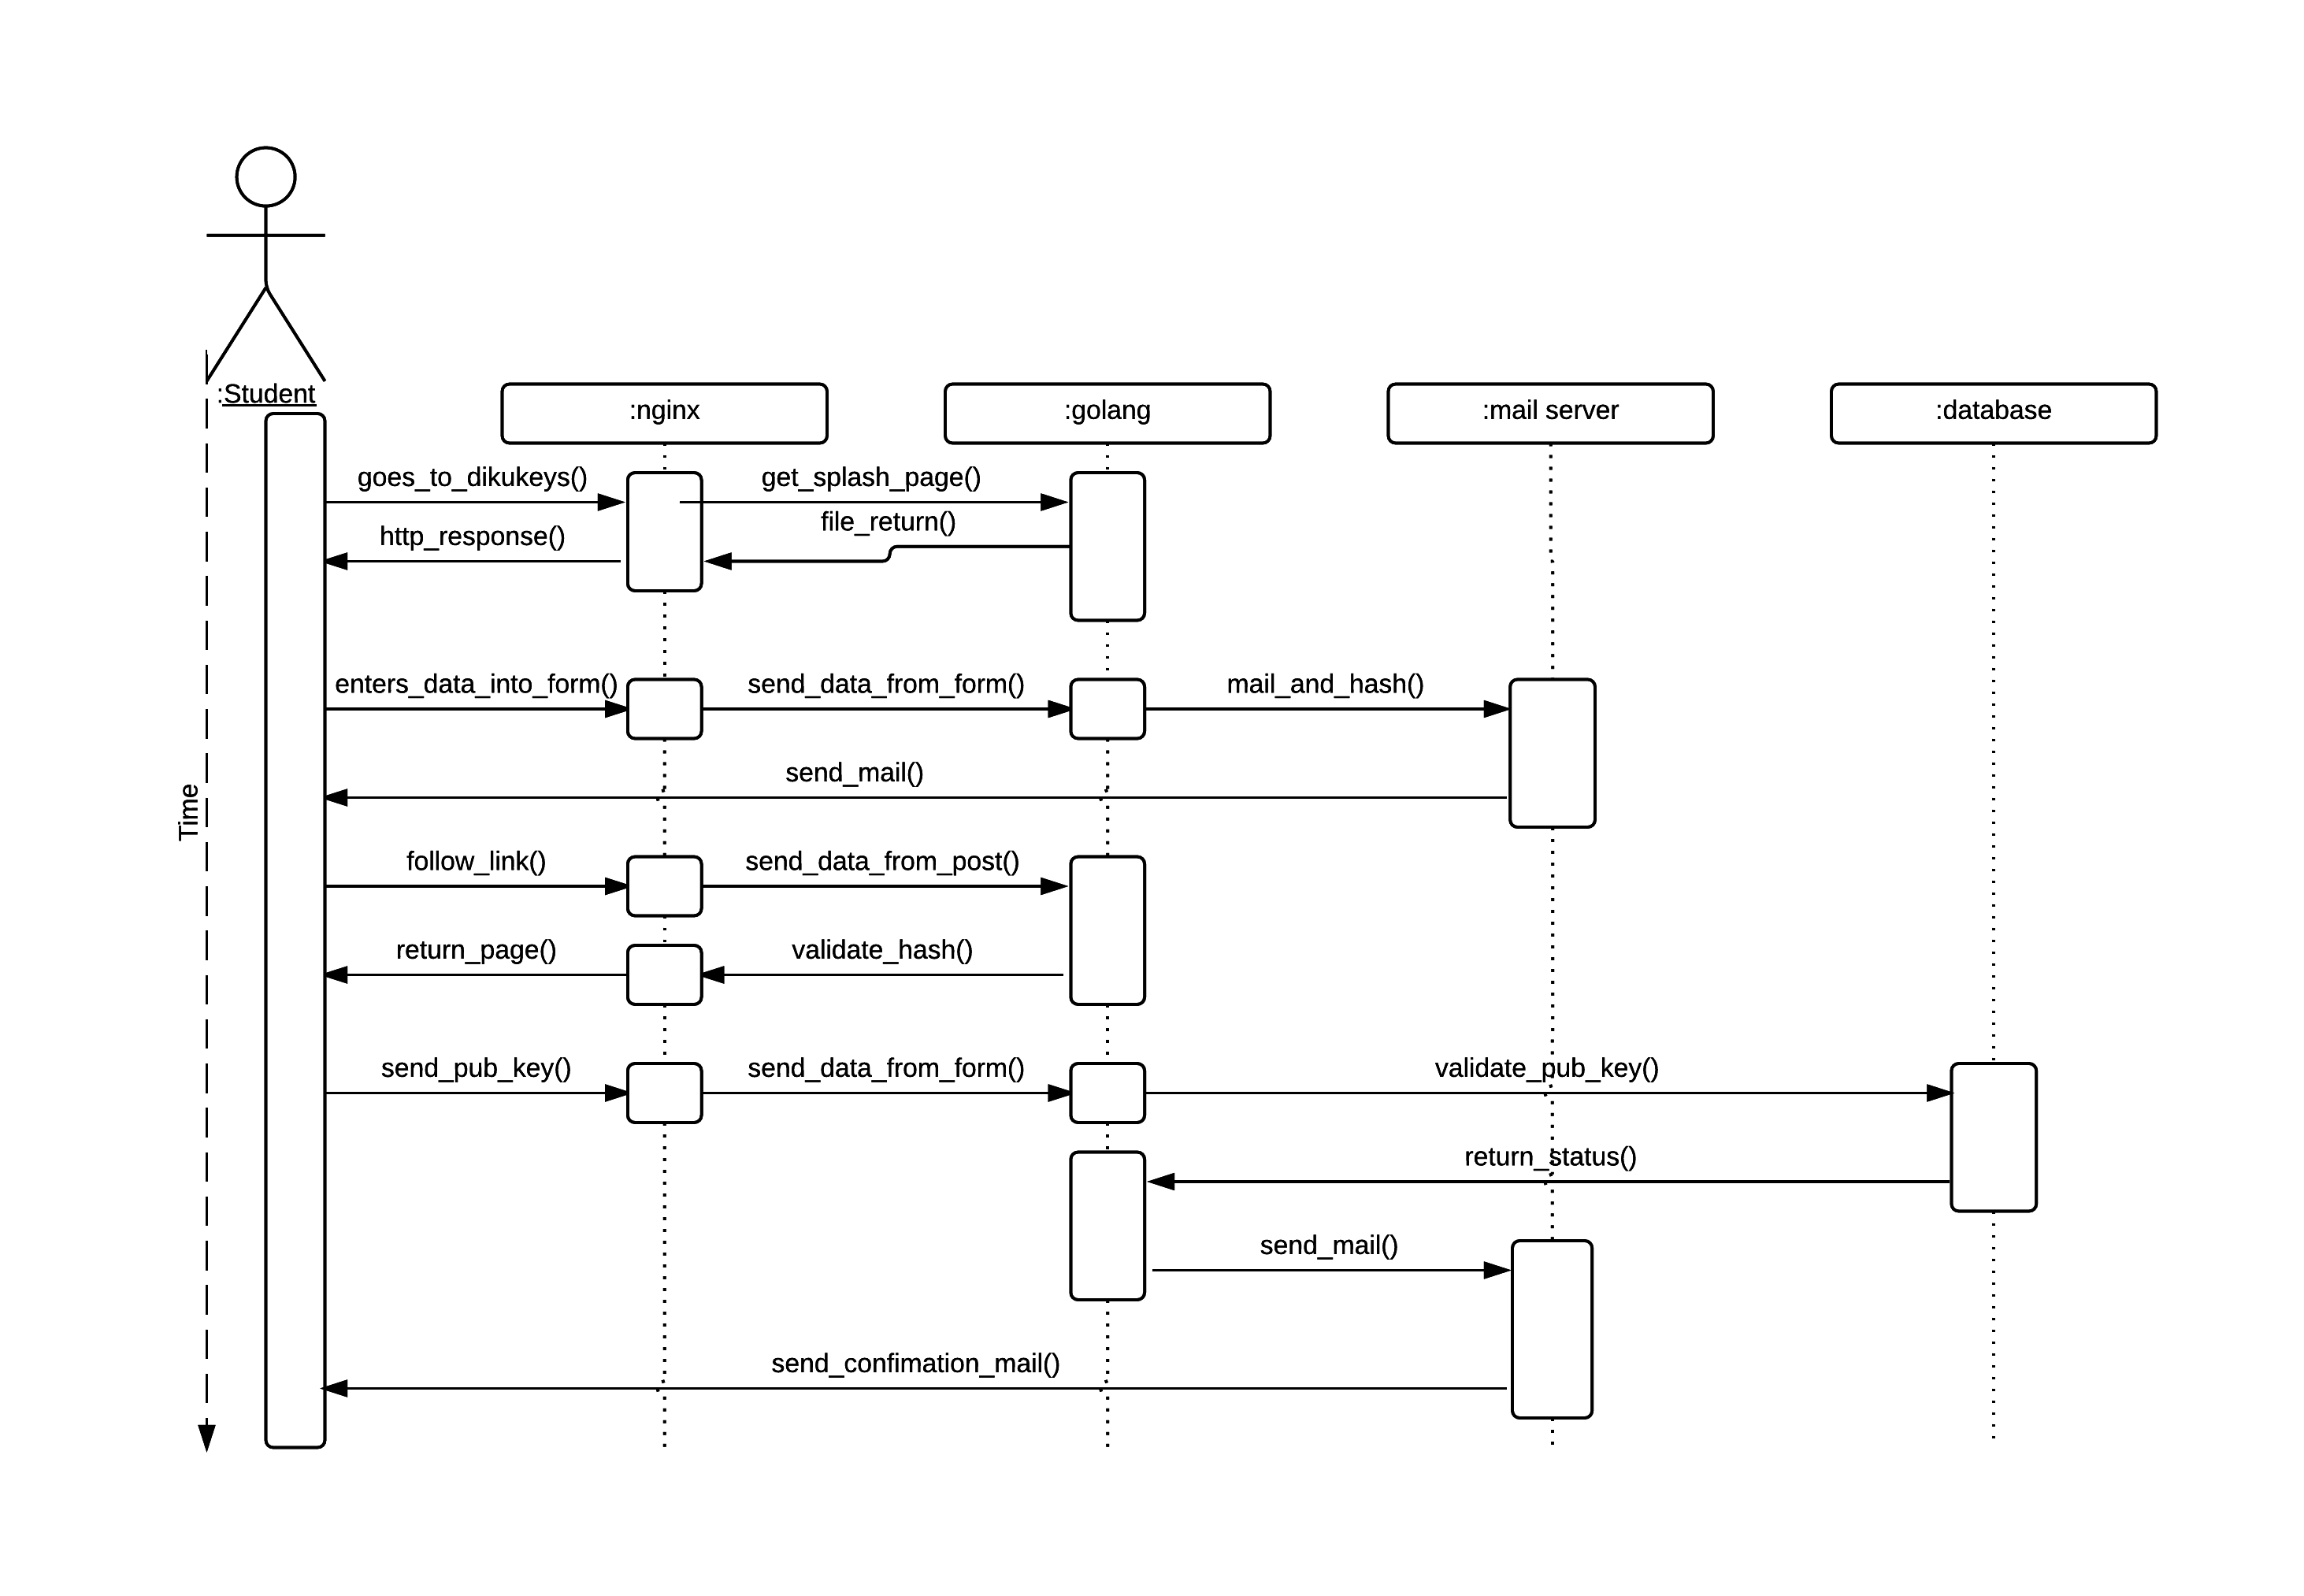
\includegraphics[width=\textwidth]{pictures/sequence_diagram_upload}
    \caption{The sequence diagram for the uploading of a public key to the database. Only the boundary classes interact with the user and only the entity class (the database) can permanently change the state of the system.}
    \label{fig:sequence_diagram}
\end{figure}

In figure \ref{fig:use_case_diagram_example_two} we have modeled the more specific use case for uploading a key.

\begin{figure}[H]
    \centering
    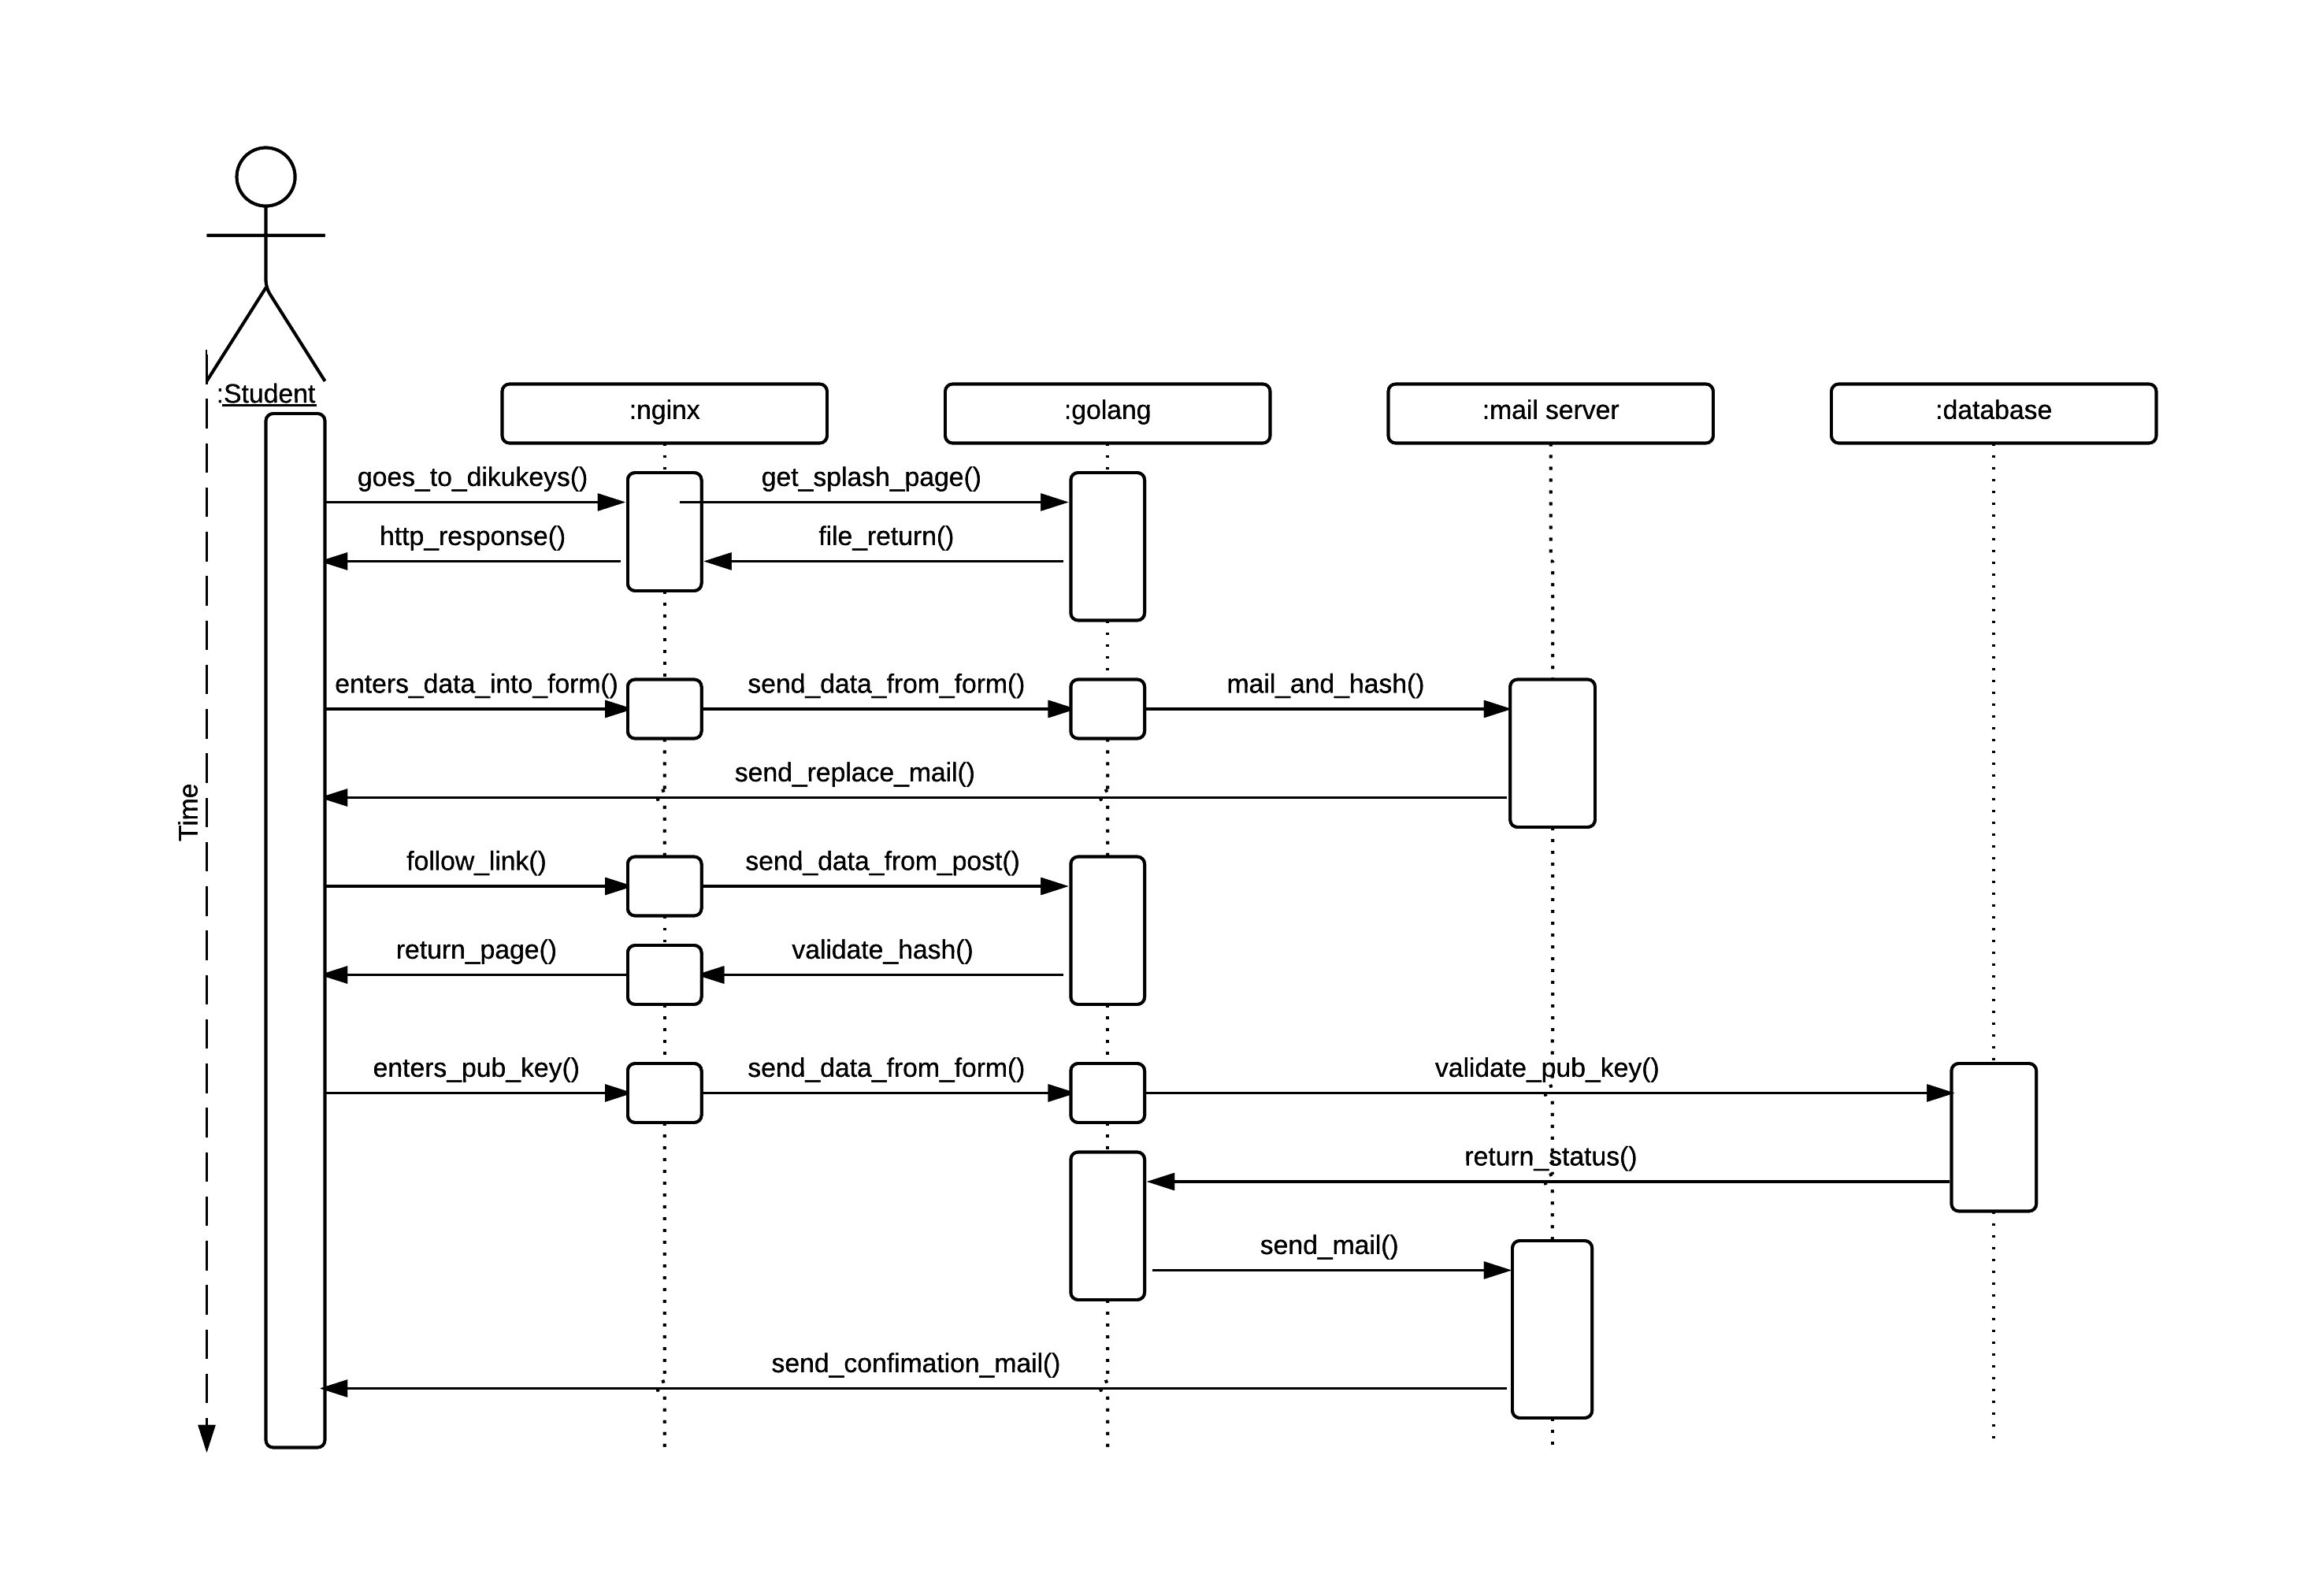
\includegraphics[width=\textwidth]{pictures/sequence_diagram_replace}
     \caption{The sequence diagram for the replacement of a public key on the database.}
    \label{fig:use_case_diagram_example_two}
\end{figure}

\section{Resumé of system design}\label{sec:Systemdesign}
\textbf{Implemented:}
\begin{itemize}
\item nginx serves as http-server and communicates with the application
through FastCGI.
\item The application communicates with postfix over SMTP to serve emails.
\end{itemize}
\textbf{Not implemented yet:}
\begin{itemize}
    \item serving a website with adaptive layout
    \item communicating with a database
    \item providing an API with authentication
\end{itemize}


\section{Program- and system tests}\label{sec:Program_systemtests}

\section{User interface and interaction design}\label{sec:UI_interactiondesign}

\section{Group Dynamics}
\subsection{What is Good?}
The knowledge level of the group seems high considering that we are \nth{1} year students. The group members complement each other well since Sven Frenzel is a smart and fast learner with an eye for detail, especially when it comes to the logic of systems. Frenzel has undertaken the vast majority of the server configuration. Mads Gram has a lot of knowledge in web-design and developing websites, in addition he has made many of the technical diagrams. Thorkil Værge has a good overview and often delegates work, while still doing a significant amount of the textual work, since his written English is remarkable.

Since the talents of the group are dissimilar, when the group works together, we are able to approach the subject from many different perspectives.

The company and social dynamics in the group are pleasant. We work very well when we are brainstorming and dividing up the work amongst ourselves.

\subsection{What is Bad?}
The work process on the \nth{2} report has not been as good as the process for the \nth{1} report since the group has not met and worked together more than one whole day. The rest of the work has been done individually or in groups of two. A better report would have been made if we had dedicated one more day to this report.

Thorkil Værge feels that we use too much time on reports and not enough time on programming and actual systems design. We do, however, learn something from all the different models for the system that we have to make.

\subsection{How can this be improved?}
To improve our work process, we should have more days where we do nothing but work on this project. Experience shows us that these days are the most effective way to work.

\newpage
\begin{appendices}
\chapter{Version Control}

We have chosen to use Git as our version control solution, this we have pared with the only git repository host GitHub.

As earlier agreed upon with our instructor Kasper Passov, we have added him to our Git repository. This will allow him to access our source code.

\href{https://github.com/Orkeren/DIKU-Keyserver/commit/5e7c7c741fbe6d2e74889e8eaff6173e8c116d46}{Inital commit on github.}

This is the initial commit with focus on our source code. It is divided into three parts, app, hash, and mail. App.go is the overarching module, which controls the web-application, the function of App.go is to interface with the web-server (nginx) and the other modules.

hash.go is a go module which enables creation of cryptographic hashes, in this iteration of the code, we only printed it to the console.  The file mail.go is another module which the code uses, this is used to send out mails, in this iteration we used it to send out a mail to our dikumail group, to show how far we were.

\href{https://github.com/Orkeren/DIKU-Keyserver/commit/690f4b0b00dc68e9b529035d7e6e6a6005072d63}{Using HTML templates commit on github.}

Earlier we used pre-encoded HTML in our app.go, with modification and extensive use of the html/template library. We were able to use html templates rather. This allows us to make changes to the pages which are displayed, without stopping the service.

\chapter{Changelog for report}

Since we use Git for our entire project, a timeline of a specific file is possible, so for our report the timeline consists of a link to a history of our document, which our document has been built from. Since we all have individual GitHub accounts, it is possible to see who committed what.

\href{https://github.com/Orkeren/DIKU-Keyserver/commits/master/docs/delrapport_2/aflevering2.tex}{Aflevering2.tex on github.}


\chapter{Timeline}
\begin{itemize}
  \item  March 16th 2015: First meeting with client, initial establishment of project. We agreed upon programming language and choice for authentication Open-PGP keys.
  \item  March 22th 2015: Second meeting with client, here we went into specifics alike API for staff and license
  \item March 29th 2015: Third meeting with client, we agreed upon using nginx as our webserver and some discussion about which database was started, but a final agreement was not reached. Lastly we agreed upon using the Bootstrap framework for the front end design. We setup a test server the same day, and got our first prototype ready.
\end{itemize}

\chapter{Minutes}
\section{Minutes from March 16th 2015}
\begin{itemize}
\item Ønsker: identificer studerende ved aflevering vha gpg-nøgle
\item Ønsker: grube med gpg-nøgle og ku-mail knyttet sammen (da der stoles på at den studerende har adgang til sin email)
\item Autentificering sker igennem unikke links til ku-mail (for at lægge gpg-nøgle op).
\SubItem 2 muligheder: copy/paste gpg-nøgle eller generer gpg-nøglepar direkte i browseren.
\item DIKU leverer ssl-certifikat.
\item Hvorfor ikke bruge eksisterende?
\item Public index j/n?
\item modtager ukrypteret nøgle og bruger den til at verificere indholdet - bagefter checkes hashet pubkey mod databasen.
\item Arbejdsbelastning: 10 timer per person per uger
\item database: (\underline{ku-nummerplade},hash(pubkey))
\end{itemize}
\subsubsection{Krav:}
\begin{itemize}
\item registrering gennem webformular og/eller kommandelinje
\item skal kunne genregistrering
\item anmodning kodkendes igennem ku-email
\item kunne vælge om den offentlige nøgle offentliggøres
\SubItem private by default
\item private API: få offentlig nøgle og returner brugernavn (kun adgang til DIKU-ansatte)
\item Sprog
\SubItem Backend: golang + sql
\SubItem frontend: html5 + js
\end{itemize}

næste møde:
2015-03-22 kl 11-16

\section{Minutes from March 22nd 2015}
The meeting was held to align the expectations of the client and the developers in regards to the systems capabilities and design.

\begin{itemize}
\item Oleks undersøger interface hvilke tilgangsmuligheder, der ønskes til databasen.
\item Kun lukket API, intet offentligt look-up. Der gemmes pupkey og abc123 (ku-brugernavn).
\item key-server i stil med MIT-keyserver er nice-to-have. Man bliver kun listet her, hvis man eksplicit ønsker dette.
\item Den studerende uploader en fil til afleveringssystemet (uden anden information). Afleveringssystemet anmoder om par af PubKey \& KU-ID og undersøger om filen er signeret af denne nøgle. Hvis ikke, så anmodes næste par indtil det korrekte par er fundet. Dette returneres til underviser.
\item Beta klar til start/midt maj.
\item Oleks gives a license (MIT-like)
\item ISA-diagram
\SubItem Fjern Admin-login fra (der er sshd-adgang til serveren anyways.)
\SubItem Front-end til client, er response og ikke request
\SubItem User guide /shell script ved ``Create key''
\item Oleks anmoder om at der sendes en dagsorden 24 timer før fremtidige møder
\item Thorkil foreslår at møder optages auditivt.
\end{itemize}

Næste møde er 29/30 marts 2015.
\end{appendices}


\begin{thebibliography}{1}

\bibitem{matthiassen} L. Mathiassen, A. Munk-Madsen, P.A. Nielsen, and J. Stage. {\em Object-Oriented Analysis \& Design} 2000: Marko Publishing House.

\bibitem{beck} Kent Beck et al. 2001 Agile Manifesto. [ONLINE] Available at: http://agilemanifesto.org/principles.html. [Accessed 19 April 15].

\bibitem{gould} Gould \& Lewis. (1985), Designing for usability: key principles and what designers think. Commun. ACM 28, 3 (March 1985), 300-311.

%\bibitem{impj}  The Japan Reader {\em Imperial Japan 1800-1945} 1973:
%Random House, N.Y.

%\bibitem{norman} E. H. Norman {\em Japan's emergence as a modern
%state} 1940: International Secretariat, Institute of Pacific
%Relations.

%\bibitem{fo} Bob Tadashi Wakabayashi {\em Anti-Foreignism and Western
%Learning in Early-Modern Japan} 1986: Harvard University Press.

\end{thebibliography}



\end{document}
